% =====================================================================
%  Surrogate-Accelerated Conjunction Assessment
%  Short report / arXiv-style preprint
%
%      pdflatex report.tex
%
%  Figures live in figures/ and are produced by src/make_figures.py.
%  The running project log (methods, failures, every measured number) is
%  project_log.tex; this file is the report drawn from it.
% =====================================================================
\documentclass[11pt]{article}

\usepackage[margin=1.1in]{geometry}
\usepackage{amsmath,amssymb}
\usepackage{booktabs}
\usepackage{graphicx}
\usepackage{siunitx}
\usepackage{multirow}
\usepackage[hidelinks]{hyperref}
\usepackage{caption}
\captionsetup{font=small,labelfont=bf}

\newcommand{\Pc}{P_c}

\title{\textbf{Surrogate-Accelerated Conjunction Assessment}\\[2pt]
\large Space-filling designs and Gaussian-process emulation for collision
probability at catalog scale, with 6-DOF dynamics and EKF/UKF orbit
determination}
\author{Anurag Paudel\\
\small Department of Applied Mathematics, University of California, Merced}
\date{September 2026}

\begin{document}
\maketitle

\begin{abstract}
Screening the tracked-object catalog for collision risk requires evaluating
collision probability $\Pc$ for every close approach, and the standard
Monte Carlo estimator is prohibitively expensive for the rare-event
probabilities involved. We show that it is worse than expensive: across the
realistic parameter range, $\Pc$ spans roughly thirteen orders of magnitude,
and at $10^{8}$ samples brute force returns \emph{zero hits} -- no estimate
at all -- for about three quarters of encounters. We build a Gaussian-process
surrogate over the encounter-parameter space, trained at points chosen by
parallel-tempering space-filling designs. Two exact invariances of the
collision integral reduce its natural six-parameter description to four, a
reduction verified numerically to $\sim10^{-12}$ and worth an
\numrange{8}{14}-fold saving in expensive evaluations. The surrogate attains
\num{0.03} orders of magnitude RMSE in $\log_{10}\Pc$ from 64 training runs
and answers subsequent queries in \SI{8}{\micro\second}, breaking even
against Monte Carlo after 64 conjunctions and running
$\sim$\num{5300} times cheaper over a \num{337789}-pair catalog screen. We
report two negative results: space-filling designs cannot be substituted for
Monte Carlo samples in the rare-event integral itself, and the
$2$--$3\times$ advantage optimised designs hold on their own criterion does
not translate into a proportional accuracy advantage.
The uncertainty above is synthesized, because the public feed carries no
covariance; the second half of the report builds the machinery that would
measure it instead. We implement a 6-DOF rigid-body propagator, validated
against closed-form torque-free precession to \SI{2e-11}{\radian} and
against conservation laws to \num{2e-13}, and compare an extended and an
unscented Kalman filter for orbit determination on identical tracking
arcs. From TLE-grade initial uncertainty the EKF becomes
\emph{confidently wrong} -- averaged NEES \num{1019} against an acceptance
band of \numrange{5.1}{7.0} -- and we locate the failure rather than
reporting it: linear covariance propagation across a tracking gap
underestimates the variance of the most tightly known direction by a factor
of \num{400}, while per-axis uncertainties remain correct to
\SI{1}{\percent}. A six-parameter campaign over a space-filling design maps
where each filter stays consistent: the EKF at \SI{28}{\percent} of design
points, the UKF at \SI{72}{\percent}.
\end{abstract}

% =====================================================================
\section{Introduction}

Two tracked objects pass close to one another. The probability that they
collide is not a geometric question, because neither position is known
precisely. Orbit uncertainty derived from two-line element sets is of order
\SI{1}{\kilo\meter}, while the objects themselves are of order
\SI{1}{\meter} and the reported miss distances are hundreds of metres. The
uncertainty is three orders of magnitude larger than the objects and larger
than the separation being resolved, so only a probability is meaningful.

We measured this gap directly. Rebuilding 37 published conjunctions by
propagating both objects from public element sets to the time of closest
approach gave separations differing from the reported miss distance by
\SIrange{0.6}{2.0}{\kilo\meter}, against reported values of
\SIrange{0.08}{0.43}{\kilo\meter} (Section~\ref{sec:uncertainty}). Every
rebuilt separation was \emph{larger} than reported, which is the expected
consequence of adding isotropic error to a near-zero displacement: distance
is a norm, so random perturbation almost always increases it.

Catalog-scale screening compounds the problem. Megaconstellation growth is
increasing the number of screened pairs faster than compute budgets grow,
and the standard Monte Carlo estimator scales as $1/\sqrt{N}$, so a tenfold
accuracy improvement costs a hundredfold in samples.

\paragraph{Contributions.}
\begin{enumerate}
  \item A measurement of \emph{where brute force fails outright} rather than
        merely slowly (Section~\ref{sec:cost}, Figure~\ref{fig:motivation}).
  \item An exact $6 \to 4$ reduction of the encounter-parameter space,
        verified numerically rather than asserted
        (Section~\ref{sec:reduction}).
  \item A Gaussian-process surrogate trained at parallel-tempering
        space-filling design points, benchmarked against random Latin
        hypercubes and uniform sampling (Section~\ref{sec:surrogate}).
  \item A triage classifier trained on a catalog screen of \num{337789}
        conjunctions, evaluated at full recall against the baseline an
        analyst would actually use (Section~\ref{sec:triage}).
  \item Two negative results (Sections~\ref{sec:negative}
        and~\ref{sec:surrogate}) that constrain how this family of methods
        should be applied.
  \item A 6-DOF rigid-body propagator validated against closed-form
        torque-free precession and against conservation laws, with the
        quaternion norm constraint handled explicitly rather than hidden
        (Section~\ref{sec:flight}).
  \item An EKF/UKF comparison in which the EKF's loss of consistency is
        \emph{located} -- a collapse of one covariance direction during
        propagation -- and a demonstration that per-axis $3\sigma$ bounds
        fail to detect it (Section~\ref{sec:od}).
  \item A six-parameter campaign mapping where each filter remains
        consistent, executed reproducibly in parallel and in containers
        (Section~\ref{sec:campaign}).
\end{enumerate}

% =====================================================================
\section{Propagation and uncertainty}\label{sec:uncertainty}

Element sets are retrieved from CelesTrak and Space-Track and propagated
with SGP4~\cite{hoots,vallado}. TLE elements are Brouwer mean elements defined by the SGP4 theory
itself; propagating them with a general-purpose orbit integrator introduces
kilometre-level error immediately, so the element set and the propagator are
used strictly as a matched pair. Propagation was validated against the
International Space Station: mean altitude \SI{419.4}{\kilo\meter} and
period \SI{92.96}{\minute} from the elements, against
\SI{92.91}{\minute} measured independently by counting minima of geocentric
radius over three days of propagation.

The public conjunction feed carries no covariance data. It reports time of
closest approach, miss distance, object identifiers, radar cross-section
class and the originator's own probability, but no state vectors and no
covariance matrices. Uncertainty must therefore be modelled, and we state it
as an assumption rather than presenting it as a data product.

Each object is assigned a diagonal covariance in its own radial /
in-track / cross-track (RTN) frame,
\begin{equation}
  C_{\text{RTN}} = \operatorname{diag}\!\left(\sigma_R^2,\;
    (k_T\sigma_R)^2,\; (k_N\sigma_R)^2\right),
  \label{eq:cov}
\end{equation}
with anisotropy ratios fixed at $k_T = 10$, $k_N = 1.5$ and only the scale
$\sigma_R$ fitted. In-track error dominates because a small period error
integrates into a growing along-track lag. Fixing the ratios is deliberate:
a full $3\times3$ covariance per object has twelve free parameters, and the
data provides one scalar observable per event. Fitting the scale alone to
the rebuilt-versus-reported miss spread gives
\begin{equation*}
  \sigma_R = \SI{95}{\meter}, \qquad
  \sigma_T = \SI{953}{\meter}, \qquad
  \sigma_N = \SI{143}{\meter},
\end{equation*}
magnitudes consistent with published TLE accuracy and obtained from our own
measurements rather than assumed. The two objects occupy different orbital
planes, so each covariance is rotated into a common inertial frame before
the relative covariance $C = C_1 + C_2$ is formed.

\paragraph{What this model does not do.} Per-event correlation between
predicted and observed error is $-0.53$. The model reproduces the aggregate
\emph{scale} of TLE uncertainty but not the per-event ranking; it does not
identify which conjunctions are worst. A single scalar observable per event
is insufficient to constrain that, and we do not claim otherwise.

% =====================================================================
\section{Collision probability and the cost of brute force}\label{sec:cost}

At the relative speeds typical of low Earth orbit
(\SIrange{10}{15}{\kilo\meter\per\second}) an encounter lasts
milliseconds and relative motion is effectively rectilinear. The
three-dimensional problem then collapses onto the two-dimensional encounter
plane perpendicular to the relative velocity~\cite{foster,chan}, and
\begin{equation}
  \Pc = \int_{\|x\| \le R} \mathcal{N}\!\left(x;\, \mu,\, C\right)
        \,\mathrm{d}x ,
  \label{eq:pc}
\end{equation}
where $\mu$ and $C$ are the projected relative miss vector and covariance
and $R$ is the combined hard-body radius.

We implement three independent estimators of \eqref{eq:pc}: a batched Monte
Carlo sampler, polar quadrature with resolution adapted to the covariance,
and a small-disk closed form valid when $R \ll \sigma$~\cite{alfano}. Monte
Carlo and
quadrature agree within Monte Carlo error bars on every real conjunction
tested (maximum $|z| = 1.4$), which cross-validates the encounter geometry
and the sampler against each other.

\begin{figure}[htbp]
\centering
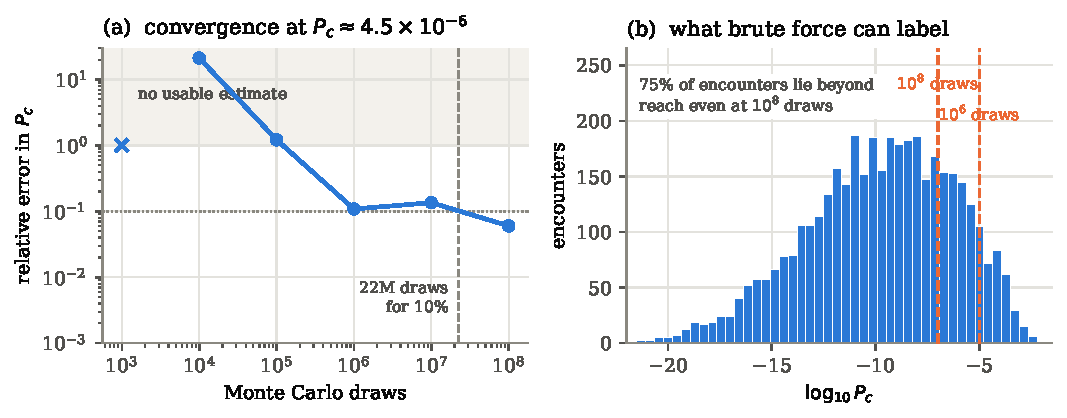
\includegraphics[width=\textwidth]{figures/fig1_motivation.pdf}
\caption{Brute force does not merely converge slowly; over most of the
parameter range it returns nothing. \textbf{(a)} Monte Carlo convergence at
a representative $\Pc \approx 4.5\times10^{-6}$: below $10^{5}$ samples the
estimator produces zero hits, and \num{22000000} samples are needed for
\SI{10}{\percent} relative error. \textbf{(b)} Distribution of $\Pc$ over
the encounter-parameter box, with the reach of two sample budgets marked at
ten expected hits. Roughly three quarters of encounters lie beyond reach
even at $10^{8}$ samples.}
\label{fig:motivation}
\end{figure}

Figure~\ref{fig:motivation} states the problem quantitatively. At
$\Pc \approx 4.5\times10^{-6}$, \num{100000} samples return \emph{zero
hits}: not a poor estimate but no estimate. Reaching \SI{10}{\percent}
relative error requires $\sim$\num{22000000} samples and \SI{1}{\percent}
requires $\sim2.2\times10^{9}$, per conjunction. Across the parameter box
$\Pc$ spans about thirteen orders of magnitude, and a substantial fraction
of encounters sit below $10^{-12}$, where no achievable sample budget yields
a single hit.

This has a direct methodological consequence: \textbf{training labels for
the surrogate cannot come from Monte Carlo}, because Monte Carlo cannot
label most of the space. We use the quadrature, which is exact in this
Gaussian setting and agrees with Monte Carlo wherever Monte Carlo works at
all. The sampler stands in for the general case -- non-Gaussian uncertainty,
long-duration encounters, non-spherical bodies -- where no closed form
exists.

% =====================================================================
\section{A negative result: designs cannot replace samples}\label{sec:negative}

The intuitive reading of ``use a space-filling design instead of Monte
Carlo'' is to replace the random samples in \eqref{eq:pc} with a
well-spread deterministic design. This does not work, and the reason is
worth stating because the idea is natural.

Equation~\eqref{eq:pc} is the integral of an indicator function over a
microscopic region. A 256-point space-filling design returns zero hits just
as $10^{5}$ random samples do, and in fact more reliably, because such a
design deliberately spreads points \emph{away} from any small region.
Quasi-Monte Carlo does not rescue the construction either: its convergence
advantage requires a smooth integrand, and an indicator over a tiny region
is the opposite of smooth.

The construction that does work places the design in the
\textbf{encounter-parameter space} rather than the sample space. Each design
point receives one expensive evaluation, a surrogate interpolates between
them, and the cost is amortised across every subsequent query.

% =====================================================================
\section{Dimensional reduction}\label{sec:reduction}

The integral \eqref{eq:pc} appears to depend on six parameters: $\mu$ (two
components), $C$ (three), and $R$ (one). Only four are independent. The
integration domain $\|x\| \le R$ is rotation-symmetric, so rotating $\mu$
and $C$ together leaves $\Pc$ unchanged; and the integral is covariant under
uniform scaling of all lengths, so dividing $\mu$, $\sqrt{C}$ and $R$ by a
common factor leaves it unchanged. Rotating into the eigenbasis of $C$ and
scaling by $R$ therefore removes two parameters, leaving
$(\mu_1/R,\, \mu_2/R,\, \sigma_1/R,\, \sigma_2/R)$.

Because a silently incorrect reduction would invalidate everything
downstream, the invariances were verified numerically rather than accepted
from the algebra (Table~\ref{tab:invariance}).

\begin{table}[htbp]
\centering
\caption{Numerical verification of the reduction over random encounters
         spanning the full parameter box. Residuals are at the level of
         quadrature noise: these are exact identities, not approximations.}
\label{tab:invariance}
\begin{tabular}{lrS[table-format=1.1e-2]}
\toprule
Claim & {Cases} & {Max.\ relative error} \\
\midrule
$\Pc$ invariant under rotation of $\mu$ and $C$ & 300 & 8.3e-13 \\
$\Pc$ invariant under uniform length scaling    & 300 & 9.8e-13 \\
Reduced form reproduces $\Pc$                   & 200 & 8.4e-13 \\
$\Pc$ even in each $\mu$ component (eigenbasis) & 200 & 6.2e-16 \\
$6 \to 4 \to \Pc$ round trip                    & 200 & 5.5e-13 \\
\bottomrule
\end{tabular}
\end{table}

The saving is substantial. Measured fill distance at $k=4$, $n=64$ is
\num{0.397}; matching it in six dimensions requires
$\sim$\numrange{500}{900} points, an \numrange{8}{14}-fold increase in
expensive evaluations for identical answers. The sign symmetry, exact to
$6\times10^{-16}$, permits restricting the domain to
$\mu_1, \mu_2 \ge 0$, reducing its volume by a further factor of four.

The identity holds \emph{given the model}: a circular hard body, Gaussian
uncertainty, and the short-term encounter approximation. Slow encounters,
below about \SI{1}{\kilo\meter\per\second} relative speed, fall outside it
and are excluded here.

% =====================================================================
\section{Surrogate}\label{sec:surrogate}

Design points are generated by parallel-tempering~\cite{geyer} optimisation
of the MaxPro criterion~\cite{joseph}, reusing the C\texttt{++}
implementation developed in our prior work on space-filling
designs~\cite{rusis} and wrapped for Python here. Designs are static artefacts: the
optimiser runs once per $(n, k)$ and costs \SIrange{0.2}{1.4}{\second}. On
its own criterion the optimised design beats the best of twenty random Latin
hypercubes~\cite{mckay} by $2.1$--$3.1\times$; the Morris--Mitchell $\phi_p$
criterion~\cite{morris} is reported alongside it in the project log.

The surrogate is a Gaussian process~\cite{rw} with an anisotropic
squared-exponential kernel, hyperparameters obtained by maximising the log marginal likelihood.
Targets are $\log_{10}\Pc$: with thirteen orders of magnitude of dynamic
range, a GP fitted to $\Pc$ itself would be dominated entirely by the few
largest values.

\begin{figure}[htbp]
\centering
\begin{minipage}[t]{0.48\textwidth}
  \centering
  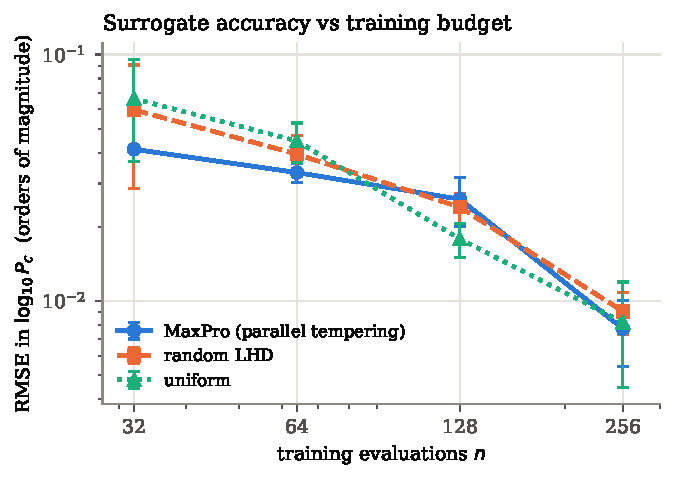
\includegraphics[width=\textwidth]{figures/fig2_surrogate.pdf}
  \caption{Surrogate accuracy against training budget, five replicates per
  design type; error bars are the standard deviation across replicates. All
  three converge by $n=256$.}
  \label{fig:surrogate}
\end{minipage}\hfill
\begin{minipage}[t]{0.48\textwidth}
  \centering
  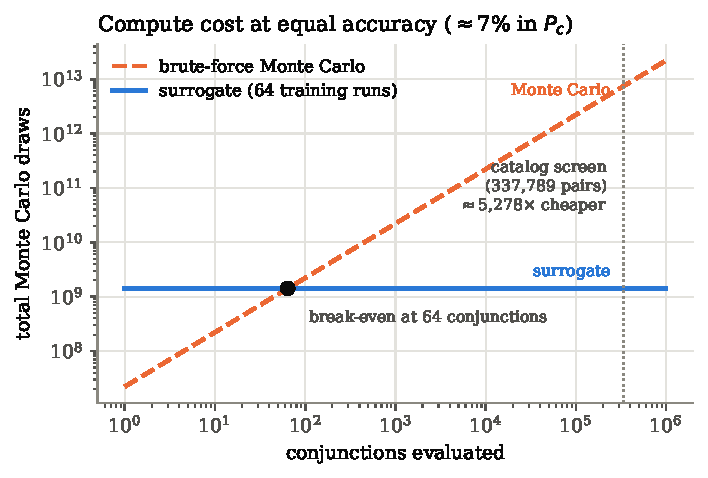
\includegraphics[width=\textwidth]{figures/fig3_cost.pdf}
  \caption{Total compute to evaluate $Q$ conjunctions at matched accuracy
  ($\approx$\SI{7}{\percent} in $\Pc$). The surrogate's cost is flat after
  training; break-even is 64 conjunctions.}
  \label{fig:cost}
\end{minipage}
\end{figure}

At $n=64$ the surrogate attains an RMSE of about \num{0.03} orders of
magnitude in $\log_{10}\Pc$ -- roughly \SI{7}{\percent} in $\Pc$ -- and
answers subsequent queries in \SI{8.3}{\micro\second}.
Figure~\ref{fig:cost} converts this into the quantity that matters at
catalog scale. Charging the surrogate its full training cost and Monte Carlo
its per-query cost at matched accuracy, the two break even at 64
conjunctions; over the \num{337789}-pair screen of
Section~\ref{sec:triage} the surrogate is $\sim$\num{5300} times cheaper.

\paragraph{A second negative result.} The $2$--$3\times$ advantage the
optimised designs hold on the MaxPro criterion \emph{does not} translate
into a proportional accuracy advantage. Mean RMSE improves by only
$1.1$--$1.8\times$ over random Latin hypercubes and uniform sampling at
$n \le 128$, and by $n=256$ the three are indistinguishable
(Figure~\ref{fig:surrogate}). The target function is smooth, so once the box
is adequately covered the design ceases to matter. Better space-filling by
the criterion is not the same thing as better surrogate accuracy.

Where the optimised designs do show a consistent advantage is
\textbf{variance}. Across replicates their RMSE spread is several times
tighter than that of random designs. With a one-shot expensive evaluation
budget a random design is a lottery -- some draws are as good as an
optimised one, others substantially worse -- and reproducibility is worth as
much to a practitioner as the mean improvement.

% =====================================================================
\section{Risk triage}\label{sec:triage}

The public conjunction feed contains no negative examples: every record is
flagged reportable with $\Pc > 10^{-4}$. A classifier trained on it learns
to answer ``yes''. We therefore manufactured negatives by screening debris
catalogs directly -- dense, co-orbital populations that generate many close
approaches per object.

Screening uses a coarse propagation grid, per-pair local minima of
separation detected on a rolling three-step window, an analytic
linear-motion filter, and parabolic refinement of the survivors. The coarse
gate must be wide: at \SI{16}{\kilo\meter\per\second} a \SI{60}{\second}
grid steps \SI{960}{\kilo\meter}, so a pair passing within
\SI{1}{\kilo\meter} may never appear closer than $\sim$\SI{450}{\kilo\meter}
at any sampled instant. The gate is consequently set to
\SI{530}{\kilo\meter}, which leaves nearly every pair a candidate; the
analytic filter, which locates the rectilinear closest approach in closed
form, then removes \SI{91}{\percent} of candidates with identical output.

The resulting dataset holds \num{337789} conjunctions from three debris
families over seven days, with 352 positives (\SI{0.104}{\percent}) at
$\log_{10}\Pc > -10$. No conjunction in this population reached the
operational $10^{-4}$ threshold, so the label threshold is a stated choice;
the ordering of methods is unchanged at $10^{-8}$ and $10^{-12}$.

Features are restricted to quantities available \emph{before} any $\Pc$
computation -- miss distance, relative speed, altitude, relative
inclination, element-set age, period difference, eccentricity and drag term.
Including $\Pc$ or anything derived from it would make the task circular.

\begin{figure}[htbp]
\centering
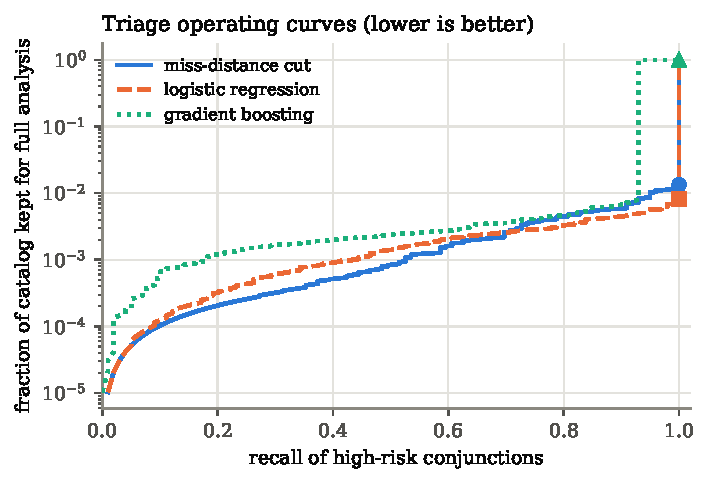
\includegraphics[width=0.62\textwidth]{figures/fig4_triage.pdf}
\caption{Triage operating curves on held-out data. Below
\SI{70}{\percent} recall a miss-distance cut is the better ranker; the
learned model wins at the high-recall end, which is the operationally
relevant one. Gradient boosting reaches full recall only by retaining the
entire catalog.}
\label{fig:triage}
\end{figure}

\begin{table}[htbp]
\centering
\caption{Triage performance. ``Kept'' is the fraction of conjunctions passed
         on for expensive analysis; lower is better at equal recall.
         Thresholds are set from out-of-fold predictions on training data
         and applied unchanged.}
\label{tab:triage}
\begin{tabular}{llrrr}
\toprule
Split & Model & Kept & Recall & Missed \\
\midrule
\multirow{3}{*}{Day}
 & Miss-distance cut (baseline) & \SI{1.41}{\percent} & \SI{100.0}{\percent} & 0 \\
 & Logistic regression          & \SI{0.92}{\percent} & \SI{100.0}{\percent} & 0 \\
 & Gradient boosting            & \SI{100.0}{\percent} & \SI{100.0}{\percent} & 0 \\
\midrule
\multirow{3}{*}{Object}
 & Miss-distance cut (baseline) & \SI{1.15}{\percent} & \SI{97.2}{\percent}  & 1 \\
 & Logistic regression          & \SI{0.82}{\percent} & \SI{100.0}{\percent} & 0 \\
 & Gradient boosting            & \SI{100.0}{\percent} & \SI{100.0}{\percent} & 0 \\
\bottomrule
\end{tabular}
\end{table}

Accuracy and AUC are near-meaningless at a \SI{0.1}{\percent} positive rate;
a constant negative prediction scores \SI{99.9}{\percent}. Because missing a
high-risk conjunction is unacceptable while passing a harmless one costs
only compute, models are compared by how much of the catalog they discard
\emph{at full recall}. The baseline is a miss-distance cut, which is what an
analyst does without a model, and splits are grouped by day or by object
rather than at random, since conjunctions in the same window share objects
and geometry.

Logistic regression passes \SIrange{0.82}{0.92}{\percent} of conjunctions
against \SIrange{1.15}{1.41}{\percent} for the baseline, and on the object
split it retains full recall where the baseline misses one. Miss distance
alone has a rank correlation of only $+0.60$ with $\log_{10}\Pc$: the
projected covariance depends on encounter geometry that a single distance
does not capture.

Gradient boosting fails outright, retaining the entire catalog under every
configuration. This is not a threshold artefact -- its oracle operating
point is also $\approx$\SI{100}{\percent}, meaning the lowest-scoring true
positive ranks below almost the whole test set. At a \SI{0.1}{\percent}
positive rate the flexible model fragments a space in which the positives
occupy a thin tail and cannot rank them, while a model whose score is
monotone in roughly the right direction can. Model capacity actively hurts.


% =====================================================================
\section{A 6-DOF rigid-body propagator}\label{sec:flight}

The covariance used in Section~\ref{sec:uncertainty} is synthesized, which
is the most serious limitation of everything above: the public feed carries
no covariance, so an error model had to be assumed and calibrated against
one scalar observable per event. An orbit-determination filter produces a
covariance \emph{from measurements} instead. Building one requires truth
trajectories from dynamics under our own control, which is what this section
supplies.

\paragraph{State and equations of motion.}
The state is thirteen elements: position $\mathbf{r}$ and velocity
$\mathbf{v}$ of the centre of mass (\si{\kilo\meter},
\si{\kilo\meter\per\second}, J2000 ECI), the attitude quaternion $q$
(scalar-first, Hamilton convention, rotating body axes into the inertial
frame), and the body angular velocity $\boldsymbol\omega$
(\si{\radian\per\second}, body axes). Translation is Newton's law per unit
mass; rotation is quaternion kinematics with Euler's equations~\cite{schaub}:
\begin{equation}
\dot{\mathbf{r}} = \mathbf{v}, \qquad
\dot{\mathbf{v}} = -\frac{\mu}{r^3}\mathbf{r} + \mathbf{a}_{J_2}, \qquad
\dot q = \tfrac12 \, q \otimes
  \begin{bmatrix} 0 \\ \boldsymbol\omega \end{bmatrix}, \qquad
I\dot{\boldsymbol\omega} = \boldsymbol\tau
  - \boldsymbol\omega \times I\boldsymbol\omega .
\label{eq:6dof}
\end{equation}
Force and torque models are supplied through a protocol; the ones
implemented are two-body gravity, the $J_2$ oblateness perturbation, and the
gravity-gradient torque
$\boldsymbol\tau_{gg} = 3\mu r^{-3}\,\hat{\mathbf u} \times I\hat{\mathbf u}$
with $\hat{\mathbf u}$ the unit radius vector in body axes. Translation and
rotation couple only through those models. Quaternion-to-matrix conversion
uses Shepperd's method~\cite{shepperd}, which stays accurate near
\SI{180}{\degree} where the naive trace formula loses all precision.

\paragraph{Integration and the norm constraint.}
A fixed-step RK4 and an adaptive DOP853~\cite{hairer} sit behind one
interface, so the two can be compared on identical problems. The exact flow
preserves $\|q\| = 1$ because $q \cdot \dot q = 0$, but a discrete
integrator does not, and the drift is handled explicitly rather than hidden
inside the equations: each integrator accepts a constraint, projects the
quaternion back to unit norm when the violation exceeds a threshold, and
reports how often it did so. DOP853 offers no hook between steps, so the
violation is detected as a terminal event, the state projected, and the
integration restarted.

\begin{table}[htbp]
\centering
\caption{Validation of the propagator. Every reference is an identity or a
         closed-form solution, not a stored output; tolerances that are not
         exact derive from a stated source of error.}
\label{tab:sixdof}
\begin{tabular}{llr}
\toprule
Check & Reference & Result \\
\midrule
Torque-free energy drift, \SI{3000}{\second}   & $T = \tfrac12 \boldsymbol\omega \cdot I \boldsymbol\omega$ conserved & \num{2.3e-13} \\
Torque-free momentum drift                     & $\mathbf{H}$ conserved as a vector & \num{5.7e-12} \\
RK4 step halving                               & fourth-order convergence & $>16\times$ reduction \\
Axisymmetric precession                        & closed form, $\dot\phi = \|H\|/I_t$ & \SI{2.3e-11}{\radian} \\
Quaternion norm, RK4 $h=\SI{0.5}{\second}$     & unit norm & \num{3.4e-7} $\to$ \num{2.2e-16} \\
Two-body orbit after one period                & closes on itself & $<\SI{1e-6}{\kilo\meter}$ \\
$J_2$ nodal regression                         & $-\tfrac32 n J_2 (R/a)^2\cos i$ & within \SI{0.42}{\percent} \\
Gravity-gradient torque                        & direct sum over point masses & \num{1e-5} \\
Small-angle pitch libration                    & $\omega = n\sqrt{3(I_2-I_1)/I_3}$ & within \SI{0.1}{\percent} \\
\bottomrule
\end{tabular}
\end{table}

Table~\ref{tab:sixdof} lists the validation; Figure~\ref{fig:sixdof} shows
the error growth behind three of its rows. Two entries deserve comment. The
quaternion norm drifts to \num{3.4e-7} unprojected and holds at
\num{2.2e-16} with projection, which is the constraint machinery earning its
place. The $J_2$ nodal rate agrees to \SI{0.42}{\percent} rather than
exactly, because the analytic rate is expressed in mean elements while the
simulation is initialised with osculating ones -- a discrepancy of order
$J_2$ itself, which is the size observed.

At matched accuracy the adaptive integrator is substantially cheaper: over
the same \SI{3000}{\second} tumble DOP853 uses \num{27200} right-hand-side
evaluations for an energy drift of \num{2.3e-13}, against \num{48000} for
RK4 at \num{1.5e-9}.

\begin{figure}[htbp]
\centering
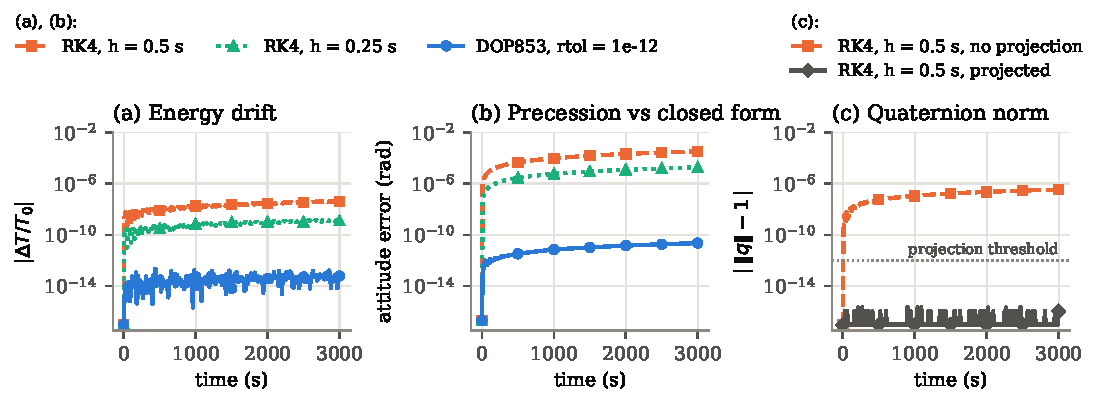
\includegraphics[width=\textwidth]{figures/fig5_6dof_validation.pdf}
\caption{Propagator validation over a \SI{3000}{\second} torque-free tumble.
(a) rotational energy drift; (b) attitude error against the closed-form
axisymmetric precession solution; (c) quaternion norm drift with and without
projection, with the projection threshold marked. Values are clamped at
\num{1e-17} so that exact zeros remain plottable on log axes.}
\label{fig:sixdof}
\end{figure}

% =====================================================================
\section{Orbit determination: EKF versus UKF}\label{sec:od}

The filter state is $x = [\mathbf{r}, \mathbf{v}]$ in J2000 ECI, propagated
with the same force models as the truth, so the comparison isolates the
filters rather than a modelling difference. The EKF propagates its
covariance with the state transition matrix obtained by integrating the
variational equations $\dot\Phi = A\Phi$ alongside the
state~\cite{montenbruck}, where the gradient $\partial \mathbf{a}/\partial
\mathbf{r}$ is taken by central differences so that a new force model needs
no hand-derived Jacobian, and uses the Joseph form of the covariance update,
which stays symmetric positive semi-definite under round-off~\cite{barshalom}.
The UKF~\cite{julier} pushes thirteen scaled sigma points~\cite{wan} through
the full nonlinear dynamics and measurement model. Its parameters are
$\alpha = 1$, $\beta = 2$, $\kappa = 0$: all weights are then non-negative
and the predicted covariance is positive semi-definite by construction,
whereas the frequently quoted $\alpha = 10^{-3}$ gives a centre weight of
about $-10^{6}$ in six dimensions.

Measurements are range and range-rate (\SI{10}{\meter},
\SI{1}{\centi\meter\per\second}) from three widely separated ground
stations with a \SI{10}{\degree} elevation mask, taken every
\SI{60}{\second} while an object is in view. Station positions are WGS-84
geodetic coordinates rotated by Greenwich mean sidereal time. Sensors are
added by implementing a measurement protocol; neither filter changes.

Consistency is judged by chi-square tests rather than by error magnitude
alone~\cite{barshalom}. The normalised estimation error squared,
$\epsilon = e^{\mathsf T} P^{-1} e$, is $\chi^2$ with six degrees of freedom
for a consistent filter; averaged over $N$ independent runs it must fall
inside a two-sided interval derived from $\chi^2(6N)/N$. An average above
the interval means the filter's covariance is too small for its own errors:
overconfident, and therefore inclined to discount the measurements that
would correct it.

\begin{table}[htbp]
\centering
\caption{Fifty Monte Carlo runs per case, two orbital revolutions, three
         stations. Only the initial uncertainty differs between cases. The
         \SI{95}{\percent} acceptance band for averaged NEES is
         \numrange{5.1}{7.0}.}
\label{tab:filters}
\begin{tabular}{llrr}
\toprule
Initial uncertainty (per axis) & Filter & {Final NEES} & {Final position RMSE} \\
\midrule
\multirow{2}{*}{\SI{10}{\meter} / \SI{1}{\centi\meter\per\second}}
 & EKF & 6.6 & \SI{3.0}{\meter} \\
 & UKF & 6.6 & \SI{3.0}{\meter} \\
\midrule
\multirow{2}{*}{\SI{1}{\kilo\meter} / \SI{1}{\meter\per\second} (TLE grade)}
 & EKF & \num{1019} & \SI{22.8}{\meter} \\
 & UKF & 8.8 & \SI{5.8}{\meter} \\
\bottomrule
\end{tabular}
\end{table}

With precise initialisation the two filters are indistinguishable and both
consistent (Table~\ref{tab:filters}). Given initial uncertainty of
\SI{1}{\kilo\meter} -- roughly what a TLE supplies, and therefore the
realistic case for the population screened in Section~\ref{sec:triage} --
the EKF's averaged NEES reaches \num{1019} and its final error is four times
the UKF's.

\paragraph{Locating the failure.} Two mechanisms contribute, and the
smaller one is the more obvious. At the first measurement update the prior
is \SIrange{1}{4}{\kilo\meter} wide, and the second-order term the EKF
discards has a standard deviation \num{3.2} times the range-rate noise
(against \num{0.36} for range); NEES rises from 5 to about 20. That is not
what produces \num{1019}. The dominant effect is in the \emph{prediction}
across the \SI{73}{\minute} gap between the first and second tracking
passes. A pass leaves the covariance extremely anisotropic, its eigenvalues
spanning some ten orders of magnitude. Second-order dynamics transfer
variance from the wide directions into the narrow ones; linear propagation
$\Phi P \Phi^{\mathsf T}$ cannot create it. Pushing a \num{4000}-point cloud
through the full nonlinear dynamics gives a smallest eigenvalue of
\num{1.5e-12}, and the UKF predicts \num{1.7e-12}, while the EKF predicts
\num{3.6e-15} -- low by a factor of \num{400}. The cloud's NEES under the
EKF covariance is \num{1104}; under the UKF's it is \num{5.3}.

The diagnostic value of this is methodological. The mean and the per-axis
radial, in-track and cross-track standard deviations agree with the true
distribution to \SI{1}{\percent} for \emph{both} filters. The EKF is wrong
only in the one direction it believes it knows best -- which is precisely the
direction NEES weights most heavily, and the direction whose small variance
causes the next measurement to be over-trusted. Consequently the customary
per-axis $3\sigma$ plot looks entirely healthy (Figure~\ref{fig:oderror})
while the averaged NEES is $150\times$ above its acceptance band
(Figure~\ref{fig:odnees}). \textbf{Plotting error against per-axis
$3\sigma$ bounds is not a consistency test.}

\begin{figure}[htbp]
\centering
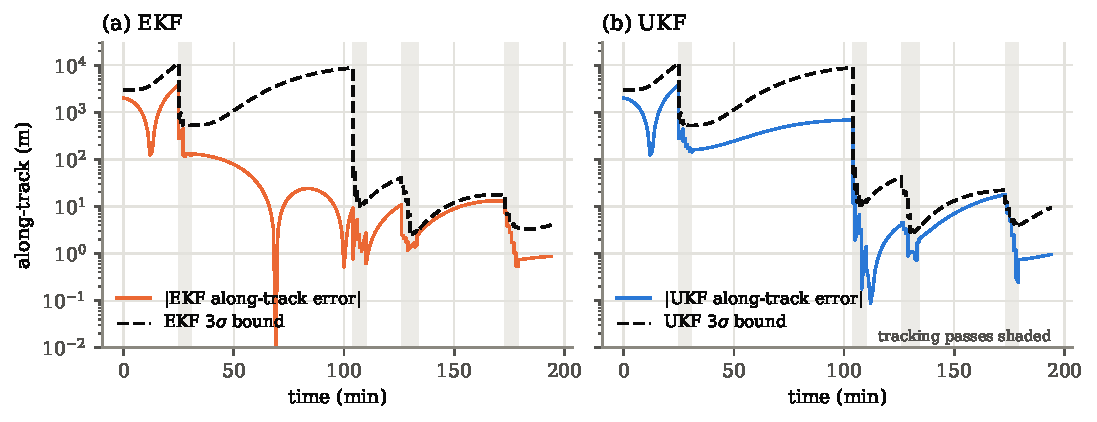
\includegraphics[width=\textwidth]{figures/fig6_estimation_error.pdf}
\caption{One run from the TLE-grade case: along-track error against the
filter's own $3\sigma$ bound, tracking passes shaded. Neither panel shows a
violation, and on this evidence both filters look sound --
Figure~\ref{fig:odnees} shows that one of them is not.}
\label{fig:oderror}
\end{figure}

\begin{figure}[htbp]
\centering
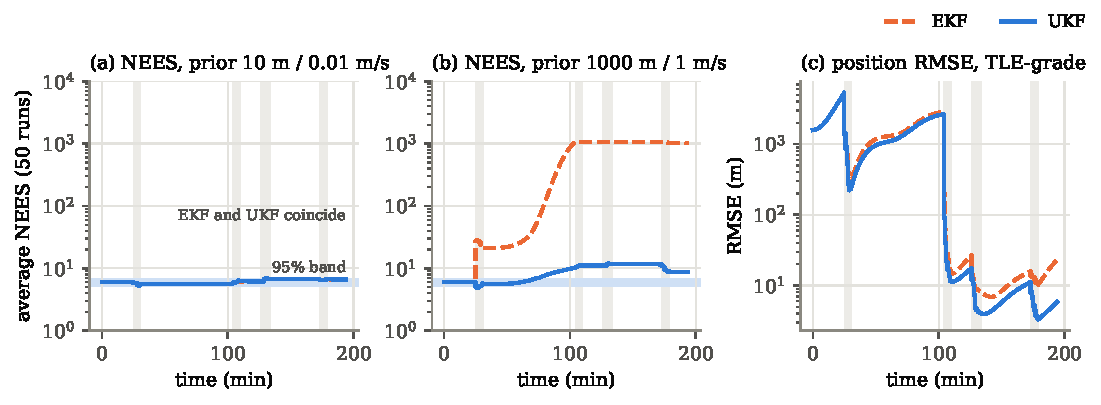
\includegraphics[width=\textwidth]{figures/fig7_estimation_consistency.pdf}
\caption{Averaged NEES over fifty runs with the \SI{95}{\percent} acceptance
band shaded, for (a) the precise prior, where the filters coincide, and
(b) the TLE-grade prior, where the EKF departs during the gap after the
first pass. (c) position RMSE for the TLE-grade case.}
\label{fig:odnees}
\end{figure}

The UKF is not vindicated unconditionally. Its averaged NEES in the
TLE-grade case settles at \num{8.8}, above the band's upper limit of
\num{7.0}: second-order moment matching is itself an approximation. The
distinction is one of kind rather than degree -- a small factor against
three orders of magnitude.

% =====================================================================
\section{Where each filter holds: a six-parameter campaign}\label{sec:campaign}

Two points in parameter space do not establish a boundary. We therefore
swept six parameters -- initial position and velocity uncertainty, range and
range-rate noise, measurement cadence, and elevation mask -- over a MaxPro
space-filling design~\cite{rusis}, the same machinery used for the surrogate
in Section~\ref{sec:surrogate}, and ran a Monte Carlo with both filters at
each of 64 design points.

\begin{table}[htbp]
\centering
\caption{Campaign over 64 design points, eight trials per point. Medians,
         because NEES spans orders of magnitude across the design and a mean
         would report only its worst points.}
\label{tab:campaign}
\begin{tabular}{lrrrr}
\toprule
Filter & {Points consistent} & {Median NEES} & {90th pct.\ NEES} & {Median RMSE} \\
\midrule
EKF & \SI{28}{\percent} & \num{70.2} & \num{1.4e8} & \SI{10.4}{\meter} \\
UKF & \SI{72}{\percent} & \num{7.0}  & \num{12.5}  & \SI{3.0}{\meter} \\
\bottomrule
\end{tabular}
\end{table}

The sweep converts the two-point result into a trend
(Figure~\ref{fig:campaign}). Binned by initial position uncertainty over
decades from \SI{10}{\meter} to \SI{10}{\kilo\meter}, the EKF is consistent
at \SI{50}{\percent}, \SI{38}{\percent}, \SI{19}{\percent} and
\SI{6}{\percent} of points, while the UKF stays near \SI{75}{\percent}
throughout. The accuracy penalty has the same shape: the median ratio of
final position error, EKF over UKF, is \num{1.30}, but the 90th percentile
is \num{1.7e3}, because beyond roughly \SI{2}{\kilo\meter} of prior
uncertainty some EKF runs diverge outright instead of degrading. Over the
whole design the UKF's worst case is NEES \num{32} and \SI{185}{\meter};
the EKF's is \num{2e17} and \SI{2570}{\kilo\meter}. Panel~(c) of
Figure~\ref{fig:campaign} shows the failures organised by prior width rather
than by sensor noise, which is the practically useful statement: it is the
quality of the initial orbit, not the quality of the radar, that decides
whether the cheaper filter is safe.

\begin{figure}[htbp]
\centering
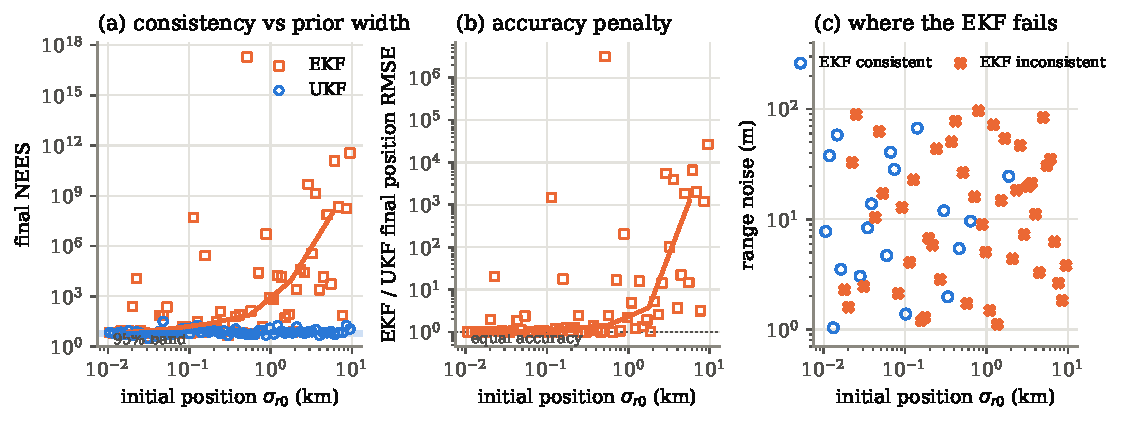
\includegraphics[width=\textwidth]{figures/fig8_campaign.pdf}
\caption{Campaign results. (a) final NEES against initial position
uncertainty, with the acceptance band shaded and binned medians overlaid;
(b) ratio of final position RMSE, EKF over UKF; (c) design points at which
the EKF is and is not consistent, against prior width and range noise.}
\label{fig:campaign}
\end{figure}

\paragraph{Reproducibility as an engineering property.} Each design point
derives its random stream from the pair (campaign seed, point index), so
results do not depend on the number of worker processes, the number of
shards, or the order in which they finish. The campaign runs locally across
cores and, unchanged, as an array job on a batch service, with the shard
index read from the environment. A two-shard, two-worker run inside the
container is bit-identical to a single-worker unsharded run; across
platforms the agreement is about $10^{-5}$ relative, because the two link
different BLAS implementations. Raw rows are persisted as Parquet beside the
configuration that produced them, its hash, and the library versions.

% =====================================================================
\section{Limitations}

\begin{enumerate}
  \item \textbf{Absolute probabilities are not validated.} Our $\Pc$ values
        run $10$--$100\times$ below the originator's published figures. The
        dominant suspect is the hard-body radius, since
        $\Pc \propto R^2$ and radar-cross-section-derived radii of
        \SIrange{1}{4}{\meter} are likely below operational values.
        Agreement with published probabilities is not claimed as validation.
  \item \textbf{Uncertainty is synthesized, not measured}, and reproduces
        the aggregate scale of TLE error rather than its per-event
        variation.
  \item \textbf{The triage population is debris}, which is small,
        uncontrolled and co-orbital; operational payload conjunctions
        differ. Test sets contain 36--99 positives, so differences of a few
        tenths of a percent should not be over-read.
  \item \textbf{Seven-day propagation from a single epoch} exceeds the
        \numrange{2}{5}-day range over which the covariance model was
        calibrated.
  \item \textbf{The dimensional reduction is model-conditional} and does not
        extend to non-Gaussian uncertainty, non-circular bodies, or
        long-duration encounters.
  \item \textbf{The two halves of this report are not yet coupled.} SGP4
        outputs TEME while the 6-DOF dynamics work in J2000 ECI, and the
        conversion between them is deliberately not implemented, so no state
        crosses from one to the other. The frames differ by the equation of
        the equinoxes -- hundreds of metres to kilometres in low Earth orbit
        -- which is precisely the scale of the uncertainty under study, so
        mixing them silently would corrupt both. Feeding a filter-derived
        covariance into $\Pc$, which is what would replace the synthesized
        model, requires that conversion first.
  \item \textbf{The Earth-orientation model is simplified.} Rotation is
        taken about the J2000 $z$-axis at the sidereal rate with Greenwich
        mean sidereal time, neglecting precession, nutation and polar motion,
        and UT1 is identified with UTC. This is self-consistent within a
        simulation, where truth and filter share it, but not adequate for
        processing real tracking data.
  \item \textbf{The estimation results contain no dynamic mismodelling.}
        Truth and filter use identical force models and the process noise is
        zero, which isolates the effect of the filters' own approximations.
        Real orbit determination also contends with unmodelled drag and
        solar radiation pressure, which this comparison does not exercise.
  \item \textbf{The UKF is not unconditionally consistent} either: it sits
        somewhat above the acceptance band in the TLE-grade case and misses
        it at about a quarter of the campaign's design points, by small
        factors rather than orders of magnitude.
\end{enumerate}

% =====================================================================
\section{Reproducibility}

All results are produced by scripts in the accompanying repository. Every
important quantity is computed two independent ways: Monte Carlo against
quadrature, the C\texttt{++} design criterion against a \texttt{numpy}
reimplementation (agreeing to six decimal places), the orbital period from
elements against a period measured by counting radius minima, and the state
transition matrix against finite differences and against its own
symplecticity. The test suite comprises 389 offline checks covering
\SI{96}{\percent} of package statements, and asserts physical identities --
conservation laws, closed-form solutions, exact invariances, chi-square
consistency bands -- in preference to stored values. Continuous integration
runs the suite, a linter enforcing numpy-style docstrings, a strict type
check, and a build of the campaign container on every push.

\begin{table}[htbp]
\centering
\caption{Commands reproducing each result.}
\label{tab:repro}
\begin{tabular}{ll}
\toprule
Command & Produces \\
\midrule
\texttt{python scripts/validate\_iss.py}   & Propagation validation (Sec.~\ref{sec:uncertainty}) \\
\texttt{python scripts/calibrate.py}       & Covariance calibration (Sec.~\ref{sec:uncertainty}) \\
\texttt{python scripts/run\_montecarlo.py} & Cost baseline (Sec.~\ref{sec:cost}) \\
\texttt{pytest tests/test\_paramspace.py}  & Table~\ref{tab:invariance} \\
\texttt{python scripts/run\_surrogate.py}  & Figure~\ref{fig:surrogate} \\
\texttt{python scripts/build\_dataset.py}  & Triage dataset (Sec.~\ref{sec:triage}) \\
\texttt{python scripts/run\_triage.py}     & Table~\ref{tab:triage} \\
\texttt{python scripts/validate\_6dof.py}  & Table~\ref{tab:sixdof}, Figure~\ref{fig:sixdof} \\
\texttt{python scripts/run\_estimation.py} & Table~\ref{tab:filters}, Figures~\ref{fig:oderror}--\ref{fig:odnees} \\
\texttt{python scripts/run\_campaign.py}   & Table~\ref{tab:campaign}, Figure~\ref{fig:campaign} \\
\texttt{python scripts/make\_figures.py}   & Figures~\ref{fig:motivation}--\ref{fig:triage} \\
\bottomrule
\end{tabular}
\end{table}

% =====================================================================
\begin{thebibliography}{9}
\small
\bibitem{hoots} F.~R. Hoots and R.~L. Roehrich,
  \emph{Models for Propagation of NORAD Element Sets}, Spacetrack Report
  No.~3, U.S. Air Force Aerospace Defense Command, 1980.
\bibitem{vallado} D.~A. Vallado,
  \emph{Fundamentals of Astrodynamics and Applications}, 4th ed.,
  Microcosm Press, 2013.
\bibitem{foster} J.~L. Foster and H.~S. Estes,
  \emph{A Parametric Analysis of Orbital Debris Collision Probability and
  Maneuver Rate for Space Vehicles}, NASA JSC-25898, 1992.
\bibitem{chan} K.~Chan, \emph{Spacecraft Collision Probability},
  Aerospace Press, 2008.
\bibitem{alfano} S.~Alfano, ``A Numerical Implementation of Spherical Object
  Collision Probability,'' \emph{Journal of the Astronautical Sciences},
  vol.~53, no.~1, 2005.
\bibitem{mckay} M.~D. McKay, R.~J. Beckman and W.~J. Conover, ``A Comparison
  of Three Methods for Selecting Values of Input Variables in the Analysis
  of Output from a Computer Code,'' \emph{Technometrics}, vol.~21, no.~2,
  1979.
\bibitem{morris} M.~D. Morris and T.~J. Mitchell, ``Exploratory Designs for
  Computational Experiments,'' \emph{Journal of Statistical Planning and
  Inference}, vol.~43, 1995.
\bibitem{joseph} V.~R. Joseph, E.~Gul and S.~Ba, ``Maximum Projection
  Designs for Computer Experiments,'' \emph{Biometrika}, vol.~102, no.~2,
  2015.
\bibitem{geyer} C.~J. Geyer, ``Markov Chain Monte Carlo Maximum
  Likelihood,'' in \emph{Computing Science and Statistics: Proceedings of
  the 23rd Symposium on the Interface}, 1991.
\bibitem{rw} C.~E. Rasmussen and C.~K.~I. Williams,
  \emph{Gaussian Processes for Machine Learning}, MIT Press, 2006.
\bibitem{rusis} J.~Beilis, A.~Paudel and J.~Mireles, ``Optimization of
  Parallel Tempering for Latin Hypercube Designs,'' RUSIS@IU Technical
  Report, 2025.
\bibitem{schaub} H.~Schaub and J.~L. Junkins, \emph{Analytical Mechanics of
  Space Systems}, AIAA Education Series.
\bibitem{shepperd} S.~W. Shepperd, ``Quaternion from Rotation Matrix,''
  \emph{Journal of Guidance and Control}, vol.~1, no.~3, 1978.
\bibitem{hairer} E.~Hairer, S.~P. N{\o}rsett and G.~Wanner, \emph{Solving
  Ordinary Differential Equations I: Nonstiff Problems}, 2nd ed.,
  Springer, 1993.
\bibitem{montenbruck} O.~Montenbruck and E.~Gill, \emph{Satellite Orbits:
  Models, Methods and Applications}, Springer, 2000.
\bibitem{julier} S.~J. Julier and J.~K. Uhlmann, ``Unscented Filtering and
  Nonlinear Estimation,'' \emph{Proceedings of the IEEE}, vol.~92, no.~3,
  2004.
\bibitem{wan} E.~A. Wan and R.~van~der~Merwe, ``The Unscented Kalman Filter
  for Nonlinear Estimation,'' in \emph{Proceedings of the IEEE Adaptive
  Systems for Signal Processing, Communications and Control Symposium},
  2000.
\bibitem{barshalom} Y.~Bar-Shalom, X.-R. Li and T.~Kirubarajan,
  \emph{Estimation with Applications to Tracking and Navigation}, Wiley,
  2001.
\end{thebibliography}

\end{document}
